%%% =====================================================================
%%% SOTA - Section 3: Automated page layout generation
%%% Mirrors Chapter~\ref{chapter:pagegen}. Addresses the MAIN objective and SO2.
%%% This is the CENTRAL axis of the thesis and the most extensive section.
%%% Treatment levels: 3.2 is P (pedagogical), 3.3 is D (detailed), 3.4 is I.
%%% =====================================================================

\section{Automated page generation and optimization}
\label{sec:sota-pagegen}

%%% TODO[SOTA]: opening paragraph. Resume the business motivation of
%%% \secref{sec:industrial-motivation}: assembling a single edition currently takes hours of manual
%%% editing, and the industrial requirement is a few minutes per page. Connect to the
%%% challenges "combinatorial complexity of spatial packing" and "balancing
%%% multi-objective trade-offs" of \secref{sec:multi-objective-page-generation}, and announce that this axis
%%% carries the main objective of \secref{sec:multi-objective-page-generation}.

\subsection{Layout Generation}
\label{sec:sota-layout-synthesis}

\subsubsection*{Deep generative methods}
Automated layout generation has recently been framed within the broader context of Artificial Intelligence Generated Content (AIGC), where a layout is treated as one deliverable among several kinds of content a generative system may produce~\cite{shi-2023}. Across this literature, a layout is abstracted uniformly as a set of graphical primitives, each parameterized by a bounding box and a category label $(c, x, y, w, h)$, regardless of whether the target domain is a printed document, a mobile interface, or a natural scene. Four families of deep generative architecture have been applied to this representation: autoregressive models, which cast layout generation as a sequence of conditional token predictions, later challenged by non-autoregressive alternatives that predict and refine every attribute in parallel instead (LayoutTransformer~\cite{gupta_layouttransformer_2021}; BLT~\cite{kong-2022}); variational autoencoders, which learn a continuous latent space over complete layouts, often paired with a graph neural network to condition generation on structural relations between elements (Neural Design Network~\cite{Lee-2020}); generative adversarial networks, in which a generator and a discriminator are trained jointly, whether searched directly in latent space under explicit constraints (CLG-LO~\cite{kikuchi-2021}) or conditioned on the content to be laid out (ContentGAN~\cite{zheng-2019}); and, more recently, flow-based and diffusion models, which generate and edit layouts through iterative denoising or bijective mappings~\cite{shi-2023}.

Most of these architectures share the underlying representation of a layout element as a bounding box tied to a category label, $(c, x, y, w, h)$, which is essentially the representation this thesis also adopts for an article placed on a page. The task posed over that shared representation, however, differs fundamentally: every system reviewed above generates the geometry itself, sampling or decoding a plausible arrangement of boxes from a learned distribution, whereas this thesis never synthesizes new boxes. Instead, within a single evolutionary search, it jointly assigns one pre-existing template, drawn from a fixed, though extensive, catalog, to each article, and packs the resulting fixed-size blocks onto the canvas, treating several explicit, conflicting editorial criteria as a Pareto trade-off~\cite{pareto} rather than folding them into a single learned or latent loss.

\subsubsection*{Rule and optimization-based methods}

A different line of work treats layout as an explicit optimization or constraint-satisfaction problem instead of something to be learned. GRIDS~\cite{Dayama-2020} formulates interactive grid-based interface layout as a mixed-integer linear program, encoding alignment, packing, and overall shape directly as objectives and constraints, and additionally samples diverse near-optimal solutions to that same program to offer a designer several alternatives rather than a single one. Jacobs et al.~\cite{jacobs-2003} address adaptive document layout with a library of hand-built, page-level grid templates, pairing each page template with a batch of content and separately allocating that content across pages through constraint solving. Note that the template here denotes an entire page rather than a single article, and pairing and allocation are resolved as two distinct steps rather than one joint decision, which sets this system apart from the per-article, jointly evolved assignment used in this thesis despite the superficial similarity of the term. More recently, LayoutRectifier~\cite{shen-2025} applies optimization as a post-process, snapping elements back onto a grid and correcting overlaps left behind by deep generative layout models.

Across these systems, geometric and perceptual criteria are formalized precisely, but each one is resolved either as a single scalarized objective or as a fixed hierarchy of constraints over a page-level unit, never as a trade-off among several conflicting editorial criteria, and never as a joint search deciding which template to assign to an article together with where to place it.

\subsubsection*{Newspaper-specific methods}

Most literature specifically targeting newspaper pages addresses segmentation of historical print for OCR rather than the generation of new layouts, which is itself telling of how little this exact problem has been studied. The few exceptions~\cite{Strecker2009AutomaticLOF, Oliveira2009TwoAFE} construct a page directly from fixed procedural rules, predating the many-objective evolutionary machinery this thesis relies on: there is no catalog of templates to select from and no search over trade-offs, since a single layout is produced deterministically and there is no objective function to trade off in the first place.

%%%%%%%%%
None of the three lines of work reviewed above matches the problem this thesis addresses, though each falls short for a different reason: the deep generative methods sample new box geometry from a learned distribution; the general-domain optimization and rule-based methods formalize objectives correctly but resolve them as a single scalarized program or a fixed constraint hierarchy over a page-level unit; and the newspaper-specific rule-based methods hand-code a deterministic procedure with no objective function at all. 

What this work does instead is to jointly assign one pre-existing template, drawn from a catalog, to each article and pack the resulting fixed-size blocks onto the canvas, within a single evolutionary search treating several conflicting editorial criteria as a multi-objective trade-off. Within this landscape, the following section narrows to multi-objective optimization, which is the framework Chapter~\ref{chapter:pagegen} adapts.

\subsection{Multi-objective optimization}
\label{sec:sota-moo}

\subsubsection*{Multi-objective problems and Pareto optimality}
\label{sec:sota-pareto}

A multi-objective optimization problem (MOP) is defined as the simultaneous minimization, or maximization, of a vector of $m \geq 2$ objective functions, $\mathbf{F}(\mathbf{x}) = (f_1(\mathbf{x}), \dots, f_m(\mathbf{x}))$, over a feasible decision space $\mathbf{x} \in \Omega$, where $\Omega$ is delimited by the problem constraints~\cite{pareto}. The map $\mathbf{F}$ sends each decision vector in $\Omega$ to a point in the objective space, and the two spaces are generally heterogeneous: a change in $\mathbf{x}$ does not translate into a proportionate change across every $f_i$. When $\Omega$ is a discrete, combinatorial set rather than a continuous region of $\mathbb{R}^n$, the problem is termed a multi-objective combinatorial optimization problem (MOCOP); this is the class instantiated in \secref{sec:objective_formulation}, where $\Omega$ ranges over feasible template and position assignments and $\mathbf{F} = \objvector{\solution}$.

A decision vector $\mathbf{x}_1 \in \Omega$ is said to dominate another vector $\mathbf{x}_2 \in \Omega$, written $\mathbf{x}_1 \preceq \mathbf{x}_2$, if $f_i(\mathbf{x}_1) \leq f_i(\mathbf{x}_2)$ for every objective $i$ and $f_j(\mathbf{x}_1) < f_j(\mathbf{x}_2)$ for at least one $j$~\cite{pareto}. A vector is non-dominated when no other feasible vector dominates it, and the Pareto-optimal set $P^\ast \subseteq \Omega$ collects every such non-dominated vector; its image $\mathbf{F}(P^\ast)$ in the objective space is the Pareto front, also referred to as the Pareto-optimal frontier. It corresponds to the boundary of trade-off compromises the problem admits, since improving one objective along $P^\ast$ necessarily worsens at least one other.

Characterizing this front in practice relies on two reference points that box it in: the ideal point $z^\ast = (z_1^\ast, \dots, z_m^\ast)$, where each $z_i^\ast = \min_{\mathbf{x} \in \Omega} f_i(\mathbf{x})$ is the best value objective $i$ attains in isolation, and the nadir point $z^{\mathrm{nad}}$, whose components are the worst value each objective takes over the Pareto-optimal set~\cite{pareto, wang-2017}. Together, $z^\ast$ and $z^{\mathrm{nad}}$ delimit the region of the objective space within which the Pareto front lies (\figref{fig:sota-pareto-front}).

Finding a single, tractable solution in the Pareto front is not straightforward. The standard approach, weighted-sum scalarization, collapses $\mathbf{F}(\mathbf{x})$ into a single scalar $\sum_{i=1}^m w_i f_i(\mathbf{x})$ and optimizes it directly, but the reduction fails for two reasons: geometrically, for a fixed weight vector $\mathbf{w}$ the minimizer coincides with a solution on the convex hull of the Pareto front, so solutions lying in non-convex regions can never be reached, regardless of how $\mathbf{w}$ is chosen~\cite{chiandussi-2012}; additionally, since objectives are conflicting, no single $\mathbf{w}$ reflects an agreed-upon priority among stakeholders, and small perturbations in $\mathbf{w}$ can shift the returned solution far along the front~\cite{savic_single-objective_2002}. This motivates searching for the complete front instead of a single scalarized solution.

The Pareto front is nonetheless a well-defined mathematical object, and for restricted problem classes it can be computed exactly rather than merely approximated: multiparametric programming derives it as a finite set of piecewise-affine regions over the space of scalarization parameters~\cite{pappas-2021}. However, such exact methods do not extend to the discrete, non-convex MOCOP this thesis addresses, at the scale required; approximating the front through a population of candidate solutions is therefore the natural alternative.

\begin{figure}[htbp]
    \centering
    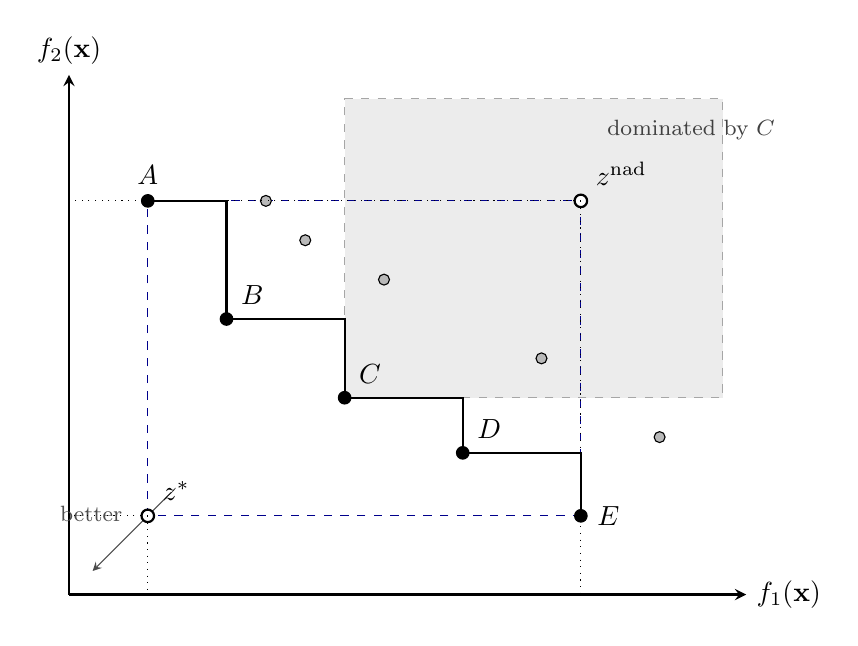
\begin{tikzpicture}[
        dominatedpt/.style={circle, fill=gray!55, draw=black, inner sep=1.4pt},
        paretopt/.style={circle, fill=black, draw=black, inner sep=1.6pt},
        refpt/.style={circle, fill=white, draw=black, thick, inner sep=1.6pt},
        >=stealth
    ]
        % Region dominated by C, shaded as a pedagogical example
        \fill[gray!15] (3.5,2.5) rectangle (8.3,6.3);
        \draw[dashed, gray!70] (3.5,2.5) rectangle (8.3,6.3);
        \node[gray!50!black, align=left] at (7.9,5.9) {\footnotesize dominated by $C$};

        % Axes
        \draw[->, thick] (0,0) -- (8.6,0) node[right] {$f_1(\mathbf{x})$};
        \draw[->, thick] (0,0) -- (0,6.6) node[above] {$f_2(\mathbf{x})$};
        \draw[->, gray!60!black] (1.3,1.3) -- (0.3,0.3) node[midway, above left, font=\footnotesize] {better};

        % Bounding box between the ideal and nadir points
        \draw[dashed, blue!55!black] (1,1) rectangle (6.5,5);

        % Pareto front: staircase through the non-dominated points
        \draw[thick] (1,5) -- (2,5) -- (2,3.5) -- (3.5,3.5) -- (3.5,2.5) -- (5,2.5) -- (5,1.8) -- (6.5,1.8) -- (6.5,1);

        % Non-dominated (Pareto-optimal) points
        \node[paretopt, label={above:$A$}] at (1,5) {};
        \node[paretopt, label={above right:$B$}] at (2,3.5) {};
        \node[paretopt, label={above right:$C$}] at (3.5,2.5) {};
        \node[paretopt, label={above right:$D$}] at (5,1.8) {};
        \node[paretopt, label={right:$E$}] at (6.5,1) {};

        % Dominated points
        \node[dominatedpt] at (2.5,5) {};
        \node[dominatedpt] at (3,4.5) {};
        \node[dominatedpt] at (4,4) {};
        \node[dominatedpt] at (6,3) {};
        \node[dominatedpt] at (7.5,2) {};

        % Ideal and nadir points, projected onto the axes
        \node[refpt, label={above right:$z^\ast$}] at (1,1) {};
        \node[refpt, label={above right:$z^{\mathrm{nad}}$}] at (6.5,5) {};
        \draw[dotted] (1,1) -- (1,0);
        \draw[dotted] (1,1) -- (0,1);
        \draw[dotted] (6.5,5) -- (6.5,0);
        \draw[dotted] (6.5,5) -- (0,5);
    \end{tikzpicture}
    \caption{Pareto dominance and the Pareto front in a bi-objective minimization problem. Black points ($A$--$E$) are non-dominated and form the Pareto front; gray points are dominated by the pareto front, and in particular every point in the shaded region is dominated by $C$. The ideal point $z^\ast$ and nadir point $z^{\mathrm{nad}}$ delimit the region containing the front.}
    \label{fig:sota-pareto-front}
\end{figure}

\subsubsection*{NSGA-II}
\label{sec:sota-emo}

Population-based evolutionary methods are naturally suited to multi-objective search: rather than converging toward a single point, a whole population of candidate solutions evolves in parallel, so that a single run can approximate the entire Pareto front instead of one trade-off at a time. Despite their algorithmic diversity, such methods share a common iterative skeleton: a population is initialized over $\Omega$, each member is evaluated through $\mathbf{F}(\mathbf{x})$, fitness is assigned according to that evaluation, variation operators generate offspring, and a selection step forms the next generation, repeating until a stopping criterion is reached~\cite{giagkiozis-2015, zhou-2011}. What distinguishes one algorithm from another is precisely how fitness assignment and selection are extended to a vector of conflicting objectives rather than a single scalar.

NSGA-II~\cite{deb-2002} instantiates this selection procedure through fast non-dominated sorting, a ranking mechanism designed to sort a population into successive levels of dominance at low computational cost. 
\begin{enumerate}
    \item For each solution $p$, the algorithm computes two quantities: $n_p$, the number of solutions that dominate $p$, and $S_p$, the set of solutions $p$ dominates.
    \item Every solution with $n_p = 0$ belongs to the first front $F_1$;
    \item The algorithm then visits each such solution $p$ and, for every solution $q \in S_p$, decrements $n_q$ by one, so that any $q$ whose count drops to zero is assigned to the next front $F_2$.
    \item  Repeating this peeling process front by front, until every solution has been assigned, sorts the whole population in $O(MN^2)$ time, where $M$ is the number of objectives and $N$ the population size.
\end{enumerate}

Beyond ranking, NSGA-II also implements a diversity-based selection mechanism, since solutions within the same front should be spread out, not clustered together. It works by measuring how crowded each solution's neighborhood is: for every objective, the solutions in a front are sorted along that objective, and the gap between a solution's two nearest neighbors is measured; summing these gaps across all objectives gives the crowding distance, so an isolated solution (i.e., with large gaps around it)scores higher than one squeezed between many similar solutions. This crowding distance improves on the density estimators used by earlier MOEAs. Solutions at the very edge of the front, with no neighbor on one side, are given an infinite distance so they are never discarded.

Together, rank and crowding distance define the crowded-comparison operator $\prec_n$: a solution $i$ is preferred over $j$ if it belongs to a better front, or, when both are in the same front, if it lies in a less crowded region. NSGA-II uses this operator to assemble the next generation:
\begin{enumerate}
    \item At every generation $t$, the parent population $P_t$ and its offspring $Q_t$ are combined into an extended population $R_t$ of size $2N$. Combining parents and offspring before selecting guarantees that no non-dominated solution found so far is ever lost, which is what makes this replacement scheme elitist.
    \item $R_t$ is sorted into fronts, as described above.
    \item The next population $P_{t+1}$ is filled front by front, from best to worst, until an entire front no longer fits within the population size $N$.
    \item The crowded-comparison operator then selects, from that last front, only as many solutions as are needed to complete $P_{t+1}$, favoring the least crowded ones.
\end{enumerate}

NSGA-III, presented next, extends this same mechanism to remain effective beyond three objectives.

\subsubsection*{NSGA-III}
\label{sec:sota-nsga3}

Beyond three objectives, non-dominated sorting alone stops providing an effective selection procedure: as the number of objectives grows, the fraction of mutually non-dominated solutions in a random population grows sharply, so that most or all of a generation ends up in the first front $F_1$, leaving the crowded-comparison operator with little left to discriminate on. This regime, conventionally termed many-objective optimization when the number of objectives ranges from about four to fifteen objectives, is exactly the one Chapter~\ref{chapter:pagegen} operates in, since it evaluates four objectives simultaneously~\cite{nsga-iii-pt1}. The crowding distance compounds the problem rather than compensating for it: estimating neighbor density becomes both more expensive and less meaningful as dimensionality increases, since most candidate solutions end up roughly as sparse as one another in a high-dimensional objective space~\cite{nsga-iii-pt1}.

NSGA-III~\cite{nsga-iii-pt1} addresses this by replacing relative density with an absolute, geometric notion of diversity, while keeping everything else from NSGA-II unchanged: the same fast non-dominated sorting, and the same elitist replacement that fills $P_{t}$ front by front. Only the last, partially admitted front is now selected differently: instead of favoring the least crowded solutions via $\prec_n$, NSGA-III associates every candidate with a predefined set of reference directions spread over the objective space, and fills the remaining slots by preserving under-represented directions rather than under-represented neighborhoods.


By default, NSGA-III generates its reference directions using the structured approach of Das and Dennis~\cite{das-dennis}, though other sampling strategies could be used instead. Each reference direction is simply a normalized weight vector $(w_1, \dots, w_M)$, one weight per objective, with $w_i \geq 0$ and $\sum_i w_i = 1$. Geometrically, the set of all such vectors forms a flat slice that cuts diagonally across the $M$ objective axes, connecting the point where $w_1=1$ (all weight on the first objective) to the equivalent point on every other axis; for $M=3$ objectives, this slice is simply the triangle joining the three axis tips shown in \figref{fig:sota-das-dennis}, and in general it is called the $(M-1)$-dimensional simplex, since fixing the weights to sum to one removes exactly one degree of freedom. Das and Dennis's construction places reference points on this slice as a regular lattice: each edge of the simplex is divided into $p$ equal parts, and a point is placed at every combination $(a_1/p, \dots, a_M/p)$ of non-negative integers $a_i$ summing to $p$, yielding exactly $H = \binom{M+p-1}{p}$ uniformly spread points. The number of divisions $p$ is therefore the only parameter controlling both the resolution and the total count of reference directions used to structure the search.



\begin{figure}[htbp]
    \centering
    \begin{tikzpicture}[refpt/.style={circle, fill=black, draw=black, inner sep=1.5pt}, >=stealth]
        % Isometric axes: f1 down-left, f2 down-right, f3 up, meeting at the origin (0,0,0)
        \draw[->, thick] (0,0) -- (-4.2,-2.42) node[left] {$f_1$};
        \draw[->, thick] (0,0) -- (4.2,-2.42) node[right] {$f_2$};
        \draw[->, thick] (0,0) -- (0,4.8) node[above] {$f_3$};

        % Axis tick marks at each division (0, 1/p, ..., 1) and the origin label
        \foreach \k in {1,2,3,4}{
            \draw (\k*-0.866,\k*-0.5) -- ++(-0.1,0.15);
            \draw (\k*0.866,\k*-0.5) -- ++(0.1,0.15);
            \draw (0,\k*1) -- ++(-0.15,0);
        }
        \node[below left, font=\scriptsize] at (0,0) {$0$};

        % Simplex triangle: the slice where w1+w2+w3=1, joining the three axis tips
        \draw[thick] (-3.464,-2) -- (3.464,-2) -- (0,4) -- cycle;

        % Internal grid lines (triangular subdivision, p=4)
        \draw[gray!50, thin] (-2.598,-0.5) -- (2.598,-0.5);
        \draw[gray!50, thin] (-1.732,1) -- (1.732,1);
        \draw[gray!50, thin] (-0.866,2.5) -- (0.866,2.5);
        \draw[gray!50, thin] (1.732,-2) -- (-0.866,2.5);
        \draw[gray!50, thin] (0,-2) -- (-1.732,1);
        \draw[gray!50, thin] (-1.732,-2) -- (-2.598,-0.5);
        \draw[gray!50, thin] (-1.732,-2) -- (0.866,2.5);
        \draw[gray!50, thin] (0,-2) -- (1.732,1);
        \draw[gray!50, thin] (1.732,-2) -- (2.598,-0.5);

        % Reference points (H = 15 lattice points on the simplex)
        \node[refpt] at (-3.464,-2) {};
        \node[refpt] at (-1.732,-2) {};
        \node[refpt] at (0,-2) {};
        \node[refpt] at (1.732,-2) {};
        \node[refpt] at (3.464,-2) {};
        \node[refpt] at (-2.598,-0.5) {};
        \node[refpt] at (-0.866,-0.5) {};
        \node[refpt] at (0.866,-0.5) {};
        \node[refpt] at (2.598,-0.5) {};
        \node[refpt] at (-1.732,1) {};
        \node[refpt] at (0,1) {};
        \node[refpt] at (1.732,1) {};
        \node[refpt] at (-0.866,2.5) {};
        \node[refpt] at (0.866,2.5) {};
        \node[refpt] at (0,4) {};

        % Annotation
        \node[align=left, font=\footnotesize] at (6.3,1) {$M=3$ objectives\\$p=4$ divisions\\$H=\binom{M+p-1}{p}=15$};
    \end{tikzpicture}
    \caption{Structured reference directions generated by the Das--Dennis construction~\protect\cite{das-dennis}, for $M=3$ objectives and $p=4$ divisions.}
    \label{fig:sota-das-dennis}
\end{figure}
Reference directions alone are not enough when objectives are measured on very different scales, since the association step described next compares distances in the objective space and would otherwise be dominated by whichever objective has the largest range. NSGA-III corrects for this at every generation through adaptive normalization~\cite{nsga-iii-pt1}: the population is translated so that the ideal point $z^\ast$ sits at the origin, and the extreme point along each objective is used to fit a hyperplane whose intercepts give the scale for that objective, so that all objectives end up comparable before distances are measured.

With every objective normalized, NSGA-III maps each population member onto the reference structure and uses that mapping to fill the remaining slots of $P_{t+1}$ from the last, partially admitted front:
\begin{enumerate}
    \item Each member is associated with the reference direction whose line, drawn from the origin, lies at the smallest perpendicular distance from it.
    \item A niche count $\rho_j$ tracks how many already-selected members are associated with each reference point $j$.
    \item Reference points with $\rho_j=0$ are prioritized first, admitting the member with the smallest perpendicular distance to that direction.
    \item Once every reference point has at least one associated member, ties are broken by selecting at random among the members associated with the least represented ones.
\end{enumerate}
This preserves diversity by spreading the population evenly across reference directions, rather than letting it accumulate around a few.




\subsubsection*{Preference-guided optimization: R-NSGA-III}
\label{sec:sota-rnsga3}

Even when non-dominance and diversity are both well preserved, the resulting Pareto front can be too large or too spread out for a decision maker to review in practice, especially as the number of objectives grows. That is the motivation to inject preference information, leting the search concentrate on the regions of the front that actually matter to the decision maker, rather than spending the same effort everywhere. 

Preferences can be articulated at three different points relative to the search: a priori, before the search begins, by supplying target values the algorithm should aim for; interactively, refining the search after inspecting an initial approximation of the front; or a posteriori, by generating the whole front first and selecting a solution from it only at the end~\cite{rnsga-iii}. Vesikar et al.~\cite{rnsga-iii} identify two situations in which a decision maker prefers this kind of local, preference-guided search over the global exploration of the entire Pareto front: (1) an iterative refinement after an initial pass, when a specific region deserves a denser set of solutions to inspect its trade-offs more closely, and (2) an a priori articulation, when domain knowledge already fixes concrete performance targets to aim for directly. Chapter~\ref{chapter:pagegen} falls into this second case, deriving its targets a priori from historical page designs.

Rather than articulating this a priori knowledge as an additional objective or constraint, R-NSGA-III~\cite{rnsga-iii} encodes it directly as one or several aspiration points $r^{(k)} = (r_1^{(k)}, \dots, r_M^{(k)})$, $k = 1, \dots, K$: target vectors in the objective space expressing the trade-off the decision maker considers desirable, without requiring that this target be attainable or even feasible. Around each aspiration point, the algorithm confines the search to a region of interest (ROI), a compact neighborhood of the objective space where the reference directions driving NSGA-III's niching mechanism (\secref{sec:sota-nsga3}) are concentrated, in place of the single, global Das-Dennis mesh. Where NSGA-III's uniform mesh treats every direction on the Pareto front as equally worth resolving, R-NSGA-III instead spends the same computational budget locally, returning a denser sample of solutions inside each ROI at the cost of coverage elsewhere.

Building the local mesh around a given aspiration point $r^{(k)}$ proceeds in four stages~\cite{rnsga-iii}:
\begin{enumerate}
    \item $r^{(k)}$ is normalized against the extreme values $f_{\min,i}$ and $f_{\max,i}$ currently attained by the population along each objective $i$, giving $\bar{r}_i^{(k)} = (r_i^{(k)} - f_{\min,i})/(f_{\max,i} - f_{\min,i})$, on the same normalized scale NSGA-III already maintains internally.
    \item $\bar{r}^{(k)}$ is projected onto the unit simplex populated by the Das-Dennis construction, yielding $\dot{r}^{(k)}$.
    \item The same $H$ Das-Dennis directions $h^{(j)}$, $j = 1, \dots, H$, used by the uniform variant for a given number of divisions $p$ are scaled by a contraction factor $\RNSGAradius \in (0,1)$, giving $\bar{h}^{(j)} = \RNSGAradius\, h^{(j)}$: since $\RNSGAradius$ multiplies coordinates measured from the simplex origin, a smaller value pulls the $H$ points into a tighter cluster, producing a denser, narrower ROI, while a value approaching $1$ leaves the mesh close in extent to the uncontracted simplex.
    \item The centroid $g$ of the contracted points $\bar{h}^{(j)}$ is computed and the whole set is translated so that this centroid coincides with the projected aspiration point, $z^{(j,k)} = \bar{h}^{(j)} + (\dot{r}^{(k)} - g)$, placing the $H$ local reference directions around $\dot{r}^{(k)}$ rather than around the simplex origin (\figref{fig:sota-aspiration-points}).
\end{enumerate}
This procedure repeats independently for every aspiration point $k=1,\dots,K$, and the $M$ extreme points of the objective space are appended to the resulting set to stabilize the adaptive normalization inherited from NSGA-III; a single run can therefore pursue several disjoint ROIs at once, the case exploited in Chapter~\ref{chapter:pagegen}.

Once the $K$ local meshes of reference directions are in place, R-NSGA-III reuses the same association and niching mechanism described for NSGA-III (\secref{sec:sota-nsga3}) unchanged. The only difference is that this selection is now carried out over directions confined to the $K$ ROIs rather than over a single global mesh, which is what concentrates selection pressure locally. At the end of the run, rather than returning the whole evolved population, R-NSGA-III filters it down to just the members closest to each of the original, uncontracted reference directions, excluding the appended extreme-point directions, handing the decision maker a compact, high-precision set of solutions instead of the entire population maintained internally by the search~\cite{rnsga-iii}.

This a priori formulation is precisely what makes aspiration points the natural vehicle for injecting the tacit editorial preference identified as a challenge in \secref{sec:multi-objective-page-generation}: professional layout practice is not codified as an explicit rule or constraint that could be added to $\Omega$, but it is observable, in aggregate, in the trade-offs historical layouts already strike across the four objectives of \secref{sec:objective_formulation}. Deriving an aspiration point directly from that historical distribution, rather than eliciting it interactively from a human operator at optimization time, lets R-NSGA-III reproduce an implicit editorial standard without ever formalizing it as an additional term in $\objvector{\solution}$.

\begin{figure}[htbp]
    \centering
    \begin{subfigure}{0.48\textwidth}
        \centering
        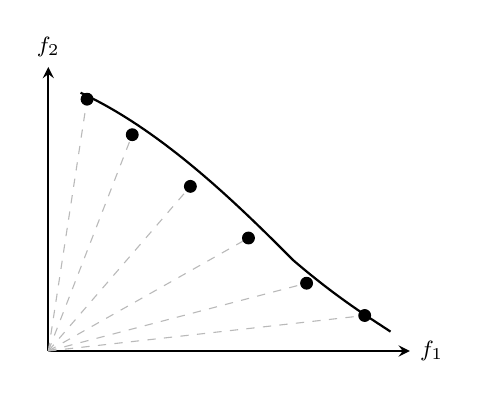
\begin{tikzpicture}[refpt/.style={circle, fill=black, draw=black, inner sep=1.5pt}, >=stealth, scale=0.82]
            \draw[->, thick] (0,0) -- (5.6,0) node[right, font=\footnotesize] {$f_1$};
            \draw[->, thick] (0,0) -- (0,4.4) node[above, font=\footnotesize] {$f_2$};

            % Pareto front
            \draw[thick] (0.5,4.0) .. controls (1.8,3.4) and (3.0,2.2) .. (3.8,1.4) .. controls (4.5,0.8) and (5.0,0.5) .. (5.3,0.3);

            % Uniform reference directions, spread over the whole front
            \foreach \p in {(0.6,3.9),(1.3,3.35),(2.2,2.55),(3.1,1.75),(4.0,1.05),(4.9,0.55)}{
                \draw[gray!55, dashed] (0,0) -- \p;
                \node[refpt] at \p {};
            }
        \end{tikzpicture}
        \caption{Uniform mesh (NSGA-III): directions are spread evenly from the origin, selecting solutions across the whole front.}
        \label{fig:sota-aspiration-points-a}
    \end{subfigure}
    \hfill
    \begin{subfigure}{0.48\textwidth}
        \centering
        \begin{tikzpicture}[refpt/.style={circle, fill=black, draw=black, inner sep=1.5pt}, asppt/.style={star, star points=5, star point ratio=2.2, fill=gray!30, draw=black, inner sep=1.6pt}, >=stealth, scale=0.82]
            \draw[->, thick] (0,0) -- (5.6,0) node[right, font=\footnotesize] {$f_1$};
            \draw[->, thick] (0,0) -- (0,4.4) node[above, font=\footnotesize] {$f_2$};

            % Pareto front, left unsampled outside the ROI
            \draw[thick, gray!45] (0.5,4.0) .. controls (1.8,3.4) and (3.0,2.2) .. (3.8,1.4) .. controls (4.5,0.8) and (5.0,0.5) .. (5.3,0.3);

            % ROI: shaded wedge contracted around the aspiration direction
            \fill[gray!20] (0,0) -- (2.85,1.95) -- (3.05,1.8) -- (3.25,1.65) -- (3.45,1.5) -- (3.65,1.35) -- cycle;

            % Local reference directions, contracted inside the ROI
            \foreach \p in {(2.85,1.95),(3.05,1.8),(3.25,1.65),(3.45,1.5),(3.65,1.35)}{
                \draw[gray!55, dashed] (0,0) -- \p;
                \node[refpt] at \p {};
            }

            % Aspiration point and its projection direction
            \node[asppt, label={below left:$r^{(k)}$}] at (2.0,1.1) {};
            \draw[dotted, thick] (0,0) -- (2.0,1.1);

            \node[font=\footnotesize] at (1.15,3.2) {ROI};
            \draw[->, gray!40!black] (1.35,2.95) to[out=-90,in=150] (2.9,2.1);
        \end{tikzpicture}
        \caption{Local mesh (R-NSGA-III): directions are contracted around an aspiration point $r^{(k)}$, concentrating solutions inside its region of interest (ROI).}
        \label{fig:sota-aspiration-points-b}
    \end{subfigure}
    \caption{Uniform reference directions of NSGA-III compared with the local directions generated around an aspiration point in R-NSGA-III~\protect\cite{rnsga-iii}. The aspiration point $r^{(k)}$ need not lie on the front itself, since it only expresses a desired trade-off. The contraction factor $\RNSGAradius$ controls how tightly the local mesh clusters around it.}
    \label{fig:sota-aspiration-points}
\end{figure}

\subsection{Two-dimensional packing}
\label{sec:sota-packing}

%%% -----------------------------------------------------------------
%%% Treatment level D (DETAILED, not a full tutorial). This is the general theoretical
%%% framework of the problem rather than a technique that the thesis adapts, so it is
%%% positioned firmly but without the pedagogical development of \secref{sec:sota-moo}.
%%% Origin: placeholder formerly at chapters/pagegen/sections/sota.tex:19.
%%% -----------------------------------------------------------------

\subsubsection*{Problem taxonomy}
\label{sec:sota-packing-taxonomy}

%%% TODO[SOTA]: to be written.
%%%  - Bin packing, strip packing and cutting stock: what distinguishes them and which
%%%    one the page generation problem reduces to.
%%%  - Guillotine versus free placement; orientation and rotation constraints.
%%%  - Situate the newspaper page: fixed canvas, heterogeneous items, no rotation,
%%%    free placement.
%%%  - Survey reference~\cite{lodi-packing-survey}.
%%% REFGAP: the formal typology of cutting and packing problems (Waescher/Dyckhoff)
%%% is absent from the bibliography and is the right anchor for this subsubsection.

\subsubsection*{Computational complexity}
\label{sec:sota-packing-complexity}

%%% TODO[SOTA]: to be written.
%%%  - NP-hardness of two-dimensional bin and strip packing.
%%%  - This subsubsection can expand on \cite{lodi-packing-survey}, already cited for
%%%    this claim in the Multi-objective page generation subsection of Chapter 1
%%%    (\secref{sec:multi-objective-page-generation}), and substantiates the challenge
%%%    "combinatorial complexity of spatial packing" stated there.
%%%  - Note the additional coupling specific to this thesis: template selection is
%%%    discrete and simultaneous with placement, which compounds the search space.

\subsubsection*{Constructive heuristics}
\label{sec:sota-packing-heuristics}

%%% TODO[SOTA]: to be written.
%%%  - Level and shelf algorithms.
%%%  - Bottom-left placement~\cite{chazelle-bl} and its efficient implementation.
%%%  - Best-fit placement for orthogonal stock cutting~\cite{burke-bf}.
%%%  - Extreme points~\cite{crainic-extreme-points}: the placement rule adopted by the
%%%    decoder of Chapter~\ref{chapter:pagegen}, so it warrants the most detail here.

\subsubsection*{Exact methods and their regime of viability}
\label{sec:sota-packing-exact}

%%% TODO[SOTA]: to be written. This subsubsection carries an argument, not just a review.
%%%  - Branch-and-bound and exhaustive backtracking for placement.
%%%  - The regime question: exact placement becomes tractable when the number of items
%%%    per instance is small. State the boundary explicitly.
%%%  - This is the direct justification for the design decision at nsga.tex:80, where an
%%%    exact backtracking decoder is preferred over a greedy heuristic because instances
%%%    involve few articles per page. The reader must be able to verify that choice from
%%%    this subsubsection.

\subsection{Learning inside optimization loops}
\label{sec:sota-surrogate}

%%% -----------------------------------------------------------------
%%% Treatment level I (INTERMEDIATE). More than plain related work, because the thesis
%%% does this, but deliberately NOT pedagogical: the surrogate was a tool, not the focus
%%% of the thesis, and should not be given the weight of \secref{sec:sota-moo}.
%%% Origin: the subsection heading formerly at chapters/pagegen/sections/sota.tex:17,
%%% which had no body.
%%% -----------------------------------------------------------------

%%% TODO[SOTA]: to be written.
%%%  - Surrogate-assisted evolutionary algorithms and fitness approximation: replacing
%%%    or complementing an expensive or unavailable objective with a learned model.
%%%  - The case relevant here is not computational cost but expressibility: the criterion
%%%    is tacit. Editorial style cannot be written analytically, so it is learned from
%%%    historical assignments. Position \neuralmethod\ in these terms, as one objective
%%%    among four, and keep it framed as a tool.
%%%  - Neural-guided population initialization and warm starts, which is the second use
%%%    made of the model in Chapter~\ref{chapter:pagegen} (see nsga.tex:221).
%%%  - Learning-to-optimize for combinatorial problems, mentioned for completeness.
%%%
%%% REFGAP (large): surrogate-assisted optimization and learning-to-optimize have no
%%% coverage in the current bibliography.

\subsection{Positioning and open gaps}
\label{sec:sota-pagegen-gaps}

%%% TODO[SOTA]: to be written. The gaps to state:
%%%  (a) Automated layout synthesis has largely treated placement and content selection
%%%      separately, whereas the industrial problem couples discrete template selection
%%%      with two-dimensional placement in a single search space.
%%%  (b) Editorial quality is not reducible to a single scalar objective, and the
%%%      criteria in play genuinely conflict, which rules out the scalarized
%%%      formulations dominant in the layout synthesis literature.
%%%  (c) Tacit editorial style has no analytical form and has not been injected as a
%%%      first-class objective into a many-objective layout generator.
%%% Close by naming Chapter~\ref{chapter:pagegen}, the main objective and SO2.
